\documentclass[nojss,article]{jss}
%              ----- for the package-vignette, don't use JSS logo, etc
%% NOTA BENE: More definitions --> further down
%%%%%%%%%%%%

%% almost as usual
\author{Marius Hofert\thanks{The first author (Willis Research Fellow) thanks
Willis Re for financial support while this paper was completed.} \\ETH Zurich
 \And
 Martin M\"achler \\ ETH Zurich}
\title{Nested Archimedean Copulas Meet \R --- The \pkg{nacopula} Package}
%% for pretty printing and a nice hypersummary also set:
\Plainauthor{Marius Hofert, Martin M\"achler} %% comma-separated
\Plaintitle{Nested Archimedean Copulas Meet R---The nacopula Package} %% without formatting
% \Shorttitle{}
%
%\VignetteIndexEntry{nacopula}
%\VignetteDepends{nacopula}
%\VignetteDepends{lattice}


%% an abstract and keywords
\Abstract{
  The package \pkg{nacopula} provides procedures for constructing
  nested Archimedean copulas in any dimensions and with any kind of nesting
  structure, generating vectors of random variates from the constructed
  objects, computing function values and probabilities of falling into
  hypercubes, as well as evaluation of characteristics such as Kendall's
  tau and the tail-dependence coefficients. As a by-product, algorithms for
  various distributions, including exponentially tilted stable
  distributions, are implemented. Detailed examples are given.
}

\Keywords{Archimedean copulas, nested Archimedean copulas, sampling algorithms,
 Kendall's tau, tail-dependence coefficients, exponentially tilted stable
 distribution, \R}
\Plainkeywords{Archimedean copulas, nested Archimedean copulas, sampling
 algorithms, Kendall's tau, tail-dependence coefficients, exponentially tilted
 stable distribution, R} %% without formatting
%% at least one keyword must be supplied

%% publication information
%% NOTE: Typically, this can be left commented and will be filled out by the technical editor
%% \Volume{13}
%% \Issue{9}
%% \Month{September}
%% \Year{2004}
%% \Submitdate{2004-09-29}
%% \Acceptdate{2004-09-29}

%% The address of (at least) one author should be given
%% in the following format:
\Address{
	Marius Hofert\\
	Department of Mathematics\\
	ETH Zurich\\
	8092 Zurich, Switzerland\\
	E-mail: \email{marius.hofert@math.ethz.ch}\\
	URL: \url{http://www.math.ethz.ch/~hofertj/}
	\par\bigskip
	Martin M\"achler\\
	Seminar f\"ur Statistik, HG G~16\\
	ETH Zurich\\
	8092 Zurich, Switzerland\\
	E-mail: \email{maechler@stat.math.ethz.ch}\\
	URL: \url{http://stat.ethz.ch/people/maechler}
}
%% It is also possible to add a telephone and fax number
%% before the e-mail in the following format:
%% Telephone: +43/1/31336-5053
%% Fax: +43/1/31336-734

%% for those who use Sweave please include the following line (with % symbols):
%% MM: this is "substituted" by  jss.cls:
%% need no \usepackage{Sweave.sty}

%% Marius' packages
\usepackage[american]{babel}%for American English
\usepackage{microtype}%for character protrusion and font expansion (only with pdflatex)
\usepackage{amsmath}%sophisticated mathematical formulas with amstex (includes \text{})
\usepackage{mathtools}%fix amsmath deficiencies
\usepackage{amssymb}%sophisticated mathematical symbols with amstex (includes \mathbb{})
\usepackage{amsthm}%theorem environments
\usepackage{bm}%for bold math symbols: \bm (= bold math)
%NON-STANDARD:\RequirePackage{bbm}%only for indicator functions
\usepackage{enumitem}%for automatic numbering of new enumerate environments
\usepackage[
  format=hang,
  labelsep=space,
  justification=justified,
  singlelinecheck=false,
  labelfont=bf
]{caption}%for captions
\usepackage{tikz}%sophisticated graphics package
\usepackage{tabularx}%for special table environment (tabularx-table)
\usepackage{booktabs}%for table layout

% This is already in jss above -- but withOUT the  fontsize=\small part !!
\DefineVerbatimEnvironment{Sinput}{Verbatim}{fontsize=\small,fontshape=sl}
\DefineVerbatimEnvironment{Soutput}{Verbatim}{fontsize=\small}
\DefineVerbatimEnvironment{Scode}{Verbatim}{fontsize=\small,fontshape=sl}

%% Marius' settings
\newcolumntype{d}[2]{D{.}{.}{#1.#2}}%aligns the entry at "." of a column if "d" is used as column type
%where the arguments specify the number of digits to the left and right for which space is kept in a column
%(always set to the maximal numbers that appear in the whole table)
\setlength{\heavyrulewidth}{0.4pt}%sets width of toprule and bottomrule in booktabs-tables
\setlength{\lightrulewidth}{0.4pt}%sets width of midrule in booktabs-tables
\setlength{\cmidrulewidth}{0.4pt}%sets width of cmidrule in booktabs-tables

%% Marius' environments
\newtheoremstyle{mythmstyle}%
	{0.5em}%space above
	{0.5em}%space below
	{}%body font
	{}%indent amount
	{\bfseries}%head font
	{}%punctuation after head
	{\newline}%space after head
	{\thmname{#1}\ \thmnumber{#2}\ \thmnote{(#3)}}%head spec
% \newcommand*{\myskip}{~\vspace{-1.2em}}%skip and space when environment begins with enumerate
\newcommand*{\myskipalgo}{~\vspace{-2.6em}}%skip and space when algorithm begins with tabbing
\newcommand*{\myskipalgotext}{~\par\vspace{-1.2em}}%skip and space when algorithm begins with text
\theoremstyle{mythmstyle}
\newtheorem{definition}{Definition}[section]%number all environments in a sequence (for every section)
\newtheorem{proposition}[definition]{Proposition}
\newtheorem{lemma}[definition]{Lemma}
\newtheorem{theorem}[definition]{Theorem}
\newtheorem{corollary}[definition]{Corollary}
\newtheorem{remark}[definition]{Remark}
\newtheorem{example}[definition]{Example}
\newtheorem{algorithm}[definition]{Algorithm}
\renewcommand*\proofname{Proof}
\makeatletter%correct qed adjustment
\renewenvironment{proof}[1][\proofname]{\par
  \pushQED{\qed}%
  \normalfont\topsep2\p@\@plus2\p@\relax
  \trivlist
  \item[\hskip\labelsep
     \sffamily\bfseries #1]~\newline\ignorespaces
}{%
  \popQED\endtrivlist\@endpefalse
}
\makeatother

\newcommand*{\R}{\proglang{R}}%{\textsf{R}}
%% Marius' commands
\newcommand*{\eps}{\varepsilon}
%NON-STANDARD{bbm}:\newcommand*{\I}{\mathbbm{1}}
\newcommand*{\I}{\mathbf{1}}
\newcommand*{\IN}{\mathbb{N}}
\newcommand*{\IK}{\mathbb{K}}
\newcommand*{\IR}{\mathbb{R}}
\newcommand*{\IC}{\mathbb{C}}
\newcommand*{\IP}{\mathbb{P}}
\newcommand*{\IE}{\mathbb{E}}
\newcommand*{\V}{\operatorname*{V}}
\newcommand*{\abs}{\operatorname*{abs}}
\renewcommand*{\S}{\operatorname*{S}}
\newcommand*{\tS}{\operatorname*{\tilde{S}}}
\newcommand*{\ran}{\operatorname*{ran}}
\newcommand*{\sgn}{\operatorname*{sgn}}
\newcommand*{\sign}{\operatorname*{sign}}
\newcommand*{\vt}{\vartheta}
\newcommand*{\vp}{\varphi}
\newcommand*{\vpi}{{\varphi^{-1}}}
\newcommand*{\vppi}{{\varphi^{[-1]}}}
\newcommand*{\psiD}{\psi^\prime}
\newcommand*{\psii}{{\psi^{-1}}}
\newcommand*{\psiis}[1]{{\psi_{#1}^{-1}}}
\renewcommand*{\L}{\mathcal{L}}
\newcommand*{\Li}{\mathcal{L}^{-1}}
\newcommand*{\LS}{\mathcal{LS}}
\newcommand*{\LSi}{\LS^{-1}}
\newcommand{\tr}{\ensuremath{^\mathsf{T}}}% or  ^{\intercal}
\renewcommand*{\O}{\mathcal{O}}
\newcommand*{\Geo}{\operatorname*{Geo}}
\newcommand*{\Exp}{\operatorname*{Exp}}
\newcommand*{\Log}{\operatorname*{Log}}
\newcommand*{\U}{\operatorname*{U}}
\newcommand*{\B}{\operatorname*{B}}
\newcommand*{\NB}{\operatorname*{NB}}
\newcommand*{\N}{\operatorname*{N}}
\newcommand*{\Var}{\operatorname*{Var}}
\newcommand*{\Cov}{\operatorname*{Cov}}
\newcommand*{\Cor}{\operatorname*{Cor}}
\hyphenation{Ar-chi-me-dean}

%% journal specific aliases
\newcommand*{\setcapwidth}[1]{}
\newcommand*{\textcite}[2][]{\citet[#1]{#2}}

%% end of declarations %%%%%%%%%%%%%%%%%%%%%%%%%%%%%%%%%%%%%%%%%%%%%%%


\begin{document}
%% include your article here, just as usual
%% Note that you should use the \pkg{}, \proglang{} and \code{} commands.
% \section[About Java]{About \proglang{Java}}
%% Note: If there is markup in \(sub)section, then it has to be escape as above.
%% Note: These are explained in '?RweaveLatex' :
\section{Introduction}
A \textit{copula} is a multivariate distribution function with standard
uniform univariate margins. Standard references for an introduction
are \textcite{joe1997} or \textcite{nelsen2007}.

\textcite{sklar1959} shows that for any multivariate
distribution function $H$ with margins $F_j$, $j\in\{1,\dots,d\}$, there exists
a copula $C$ such that
\begin{align}
	H(x_1,\dots,x_d)=C(F_1(x_1),\dots,F_d(x_d)),\ \bm{x}\in\IR^d.\label{sklar}
\end{align}
Conversely, given a copula $C$ and arbitrary univariate distribution functions $F_j$,
$j\in\{1,\dots,d\}$, $H$ defined by (\ref{sklar}) is a distribution function
with marginals $F_j$, $j\in\{1,\dots,d\}$. On one hand, Sklar's Theorem
tells us that we can decompose any given multivariate distribution function into
its margins and a copula. By this decomposition, copulas allow us to study
multivariate distributions functions independently of the margins. This is of
particular interest in statistics. On the other hand, Sklar's Theorem provides a
tool for constructing large classes of multivariate distributions and is
therefore often used for sampling multivariate distributions via
copulas. This is indispensable for
many applications in the areas of statistics and finance. For sampling the
multivariate distribution $H$ it suffices to sample the common dependence
structure, given by the copula $C$, and to transform the obtained variates to
the correct margins $F_j$, $j\in\{1,\dots,d\}$. Since this transformation is
usually easy to achieve (simply apply the \textit{generalized inverse}
$F_j^-(y):=\inf\{x\in\IR:F_j(x)\ge y\}$ corresponding to $F_j$,
$j\in\{1,\dots,d\}$, with the convention that $\inf\emptyset:=\infty$), sampling
from $H$ usually boils down to sampling the copula $C$ under consideration.

Besides elliptical copulas, Archimedean copulas play an important role in
practical applications. In contrast to elliptical ones, Archimedean copulas
are given explicitly in terms of a generator and they are able to capture
different kinds of tail dependencies, e.g., upper, but not lower tail
dependence. With the algorithm of \textcite{marshallolkin1988}, they are
also usually easy to sample. Their functional symmetry (in $u_j$,
$j=1,\dots,d$), also referred to as \textit{exchangeability}, however, is often considered to be a drawback, e.g.,
in risk-management applications where the considered portfolios are
typically high-dimensional. To circumvent exchangeability, Archimedean copulas
can be nested into each other under certain conditions. The resulting
copulas are referred to as \emph{``nested Archimedean copulas''} and allow to model
hierarchical dependence structures.

\section{Archimedean copulas}
\subsection{Archimedean copulas and their properties}
An \textit{Archimedean generator}, or simply \textit{generator}, is a
continuous, decreasing function $\psi:[0,\infty]\to[0,1]$ which satisfies
$\psi(0)=1$, $\psi(\infty):=\lim_{t\to\infty}\psi(t)=0$, and which is strictly
decreasing on $[0,\inf\{t:\psi(t)=0\}]$. A $d$-dimensional copula is called
\textit{Archimedean} if it is of the form
\begin{align}
  C(\bm{u};\psi):=\psi(\psii(u_1)+\dots+\psii(u_d)),\ \bm{u}\in[0,1]^d,\label{ac}
\end{align}
for some generator $\psi$ with inverse $\psii:[0,1]\to[0,\infty]$, where
$\psii(0):=\inf\{t:\psi(t)=0\}$. A necessary and sufficient condition for
an Archimedean generator $\psi$ to generate a proper copula in all
dimensions $d$ is that $\psi$ is \textit{completely monotone}, i.e.,
$(-1)^k\psi^{(k)}(t)\ge0$ for all $t\in(0,\infty)$ and $k\in\IN_0$, see
\textcite{kimberling1974} in the context of t-norms or
\textcite[p.\ 54]{hofert2010c} for a rework in terms of copulas.
Recall that the most simple dependence model, namely, independence, is provided
by $\psi(t)=\exp(-t)$, with $\psii(t)=\log(t)$, and corresponding
\textit{independence} copula $C({\bm u})=\prod_{j=1}^d u_j$.

The class of all completely monotone Archimedean generators is denoted by
$\Psi_\infty$ in what follows. By Bernstein's Theorem, see, e.g.,
\textcite[p.\ 439]{feller1971}, this class coincides with the class of
Laplace-Stieltjes transforms of distribution functions $F$ on the positive
real line, where the Laplace-Stieltjes transform of $F$, also known as the
\textit{Laplace transform of the distribution}, % <- hier kein $F$ (MM)
is defined as
\begin{align*}
  \LS[F](t):=\int_0^\infty\exp(-tx)\,dF(x),\ t\in[0,\infty).
\end{align*}
For a $\psi\in\Psi_\infty$, we hence have the relation
\begin{align*}
  \psi=\LS[F],\ \text{or, equivalently,}\ F=\LSi[\psi].
\end{align*}
for a distribution function $F$ on the positive real line.

Note that the distribution function $F$ is known for virtually all commonly
used Archimedean generators, see, e.g., \textcite[p.\ 62]{hofert2010c}. The
package \pkg{nacopula} currently provides the most widely used families of
Ali-Mikhail-Haq, Clayton, Frank, Gumbel, and Joe, see Table~\ref{tab:cop-families-psi}
for the generators and their corresponding distribution functions. Except
for Clayton's family, where we use a slightly simpler generator, these
generators are the ones given in \textcite[pp.\ 116]{nelsen2007}.

These Archimedean copula families are provided as \code{"acopula"} \R\
objects, containing as slots the corresponding generator
$\psi$, \code{psi}, its inverse $\psii$, \code{psiInv},
and the ``sampler'', i.e., random number generator for $V\sim F$, as \code{V0}:
\begin{Schunk}
\begin{Sinput}
> require(nacopula)
> ls("package:nacopula", pattern = "^cop[A-Z]")
\end{Sinput}
\begin{Soutput}
[1] "copAMH"     "copClayton" "copFrank"   "copGumbel"  "copJoe"    
\end{Soutput}
\begin{Sinput}
> copClayton
\end{Sinput}
\begin{Soutput}
Archimedean copula ("acopula"), family "Clayton"
 It contains further slots, named
  "psi", "psiInv", "paraConstr", "paraInterval", "V0", "tau",
  "tauInv", "lambdaL", "lambdaLInv", "lambdaU", "lambdaUInv",
  "nestConstr", "V01"
\end{Soutput}
\begin{Sinput}
> copClayton@psi
\end{Sinput}
\begin{Soutput}
function (t, theta) 
{
    (1 + t)^(-1/theta)
}
<environment: namespace:nacopula>
\end{Soutput}
\begin{Sinput}
> copClayton@psiInv # the inverse of psi(), psi^{-1}
\end{Sinput}
\begin{Soutput}
function (t, theta) 
{
    t^(-theta) - 1
}
<environment: namespace:nacopula>
\end{Soutput}
\begin{Sinput}
> copClayton@V0     # "sampler" for  V ~ F()
\end{Sinput}
\begin{Soutput}
function (n, theta) 
{
    rgamma(n, shape = 1/theta)
}
<environment: namespace:nacopula>
\end{Soutput}
\end{Schunk}
The majority of slots of such copula objects are functions, encoding properties
of that copula family. In what follows, many of these functions are presented.

\subsubsection{Sampling Archimedean copulas}
From a mixture representation with respect to $F$, the following algorithm
may be derived for sampling Archimedean copulas, see
\textcite{marshallolkin1988}.
\begin{algorithm}[\textcite{marshallolkin1988}]
  \myskipalgo
  \linespread{1.22}\normalfont
  \begin{tabbing}
    \hspace{8mm} \= \hspace{4mm} \= \kill
    (1) \> \textbf{sample} $V\sim F := \LSi[\psi]$\\
    (2)	\> \textbf{sample} $R_j\sim\Exp(1)$, $j\in\{1,\dots,d\}$\\
    (3)	\> \textbf{set} $U_j:=\psi(R_j/V)$, $j\in\{1,\dots,d\}$\\
    (4) \> \textbf{return} $\bm{U}=(U_1,\dots,U_d)\tr$
  \end{tabbing}
\end{algorithm}
In order for this algorithm to be easily applied, we need to know how to
sample the distribution functions $F=\LSi[\psi]$. For the families of
Ali-Mikhail-Haq, Clayton, Frank, Gumbel, and Joe, see
Table~\ref{tab:cop-families-psi}.
\begin{table}[htbp]
  \centering
  \begin{tabularx}{\textwidth}{@{\extracolsep{\fill}}X>{\hspace{-6mm}}cc>{\hspace{-4mm}}c}
    \toprule
    \multicolumn{1}{c}{Family}&\multicolumn{1}{c}{\hspace{-6mm}$\vt$}&\multicolumn{1}{c}{$\psi(t)$}&\multicolumn{1}{c}{\hspace{-4mm}$V\sim F=\LSi[\psi]$}\\
    \midrule
    Ali-Mikhail-Haq&$[0,1)$&$(1-\vt)/(\exp(t)-\vt)$&$\Geo(1-\vt)$\\
    Clayton&$(0,\infty)$&$(1+t)^{-{1/\vt}}$&$\Gamma(1/\vt,1)$\\
    Frank&$(0,\infty)$&$-\log(1-(1-e^{-\vt})\exp(-t))/\vt$&$\Log(1-e^{-\vt})$\\
    Gumbel&$[1,\infty)$&$\exp(-t^{1/\vt})$&$\S(1/\vt,1,\cos^\vt(\pi/(2\vt)),\I_{\{\vt=1\}};1)$\\
    Joe&$[1,\infty)$&$1-(1-\exp(-t))^{1/\vt}$&$\binom{1/\vt}{k}(-1)^{k-1},\ k\in\IN$\\
    \bottomrule
  \end{tabularx}
  \caption{Commonly used one-parameter Archimedean generators.}
  \label{tab:cop-families-psi}
\end{table}

For the family of Ali-Mikhail-Haq, $\Geo(p)$ denotes a \textit{geometric
  distribution} with success probability $p\in(0,1]$ and mass function
$p_k=p(1-p)^{k-1}$ at $k\in\IN$ (which in \R\ is \code{dgeom(}$k$,$p$\code{)}).
%
For Clayton's family, $\Gamma(\alpha,\beta)$ denotes the \textit{gamma
  distribution} with shape $\alpha\in(0,\infty)$, rate
$\beta\in(0,\infty)$, and density
$f(x)=\beta^\alpha x^{\alpha-1}\exp(-\beta x)/\Gamma(\alpha)$, $x\in(0,\infty)$
(provided in \R\ by \code{[dpqr]gamma(., shape=}$\alpha$\code{, rate=}$\beta$\code{)}).
%
For the family of Frank, $\Log(p)$ denotes a
\textit{logarithmic distribution} with parameter $p\in(0,1)$ and mass
function $p_k=p^k/(-k\log(1-p))$ at $k\in\IN$. For sampling this
distribution, we provide \code{rlog(., }$p$\code{)}, using the algorithm
``LK'' of \textcite{kemp1981}.
%
For Gumbel's family, $F$ corresponds to a $S(\alpha, \beta, \gamma, \delta; 1)$, i.e., a \textit{stable}, distribution with characteristic function
\begin{align}
	\phi(t)=\exp\bigl(i\delta t-\gamma^\alpha\lvert t\rvert^\alpha(1-i\beta\sgn(t)w(t,\alpha))\bigr),\ t\in\IR,
\end{align}
where
\begin{align*}
	w(t,\alpha)=\begin{cases}
			\tan(\alpha\pi/2),&\alpha\neq1,\\
			-2\log(\lvert t\rvert)/\pi,&\alpha=1,
		\end{cases}
\end{align*}
see, e.g., \textcite[p.\ 8]{nolan2009} for this ``1-parameterization''. For
sampling from $S(.)$, we provide
\code{rstable1(., }$\alpha$,$\beta$,$\gamma$, $\delta$\code{, 1)},
having implemented an algorithm for sampling stable distributions according
to the ideas presented in \textcite{chambersmallowsstuck1976}, and
improving on previous implementations in \R.
%
For the family of Joe, the mass function of $V$ is of the form
$p_k=\binom{\alpha}{k}(-1)^{k-1}$ at $k\in\IN$ (take $\alpha:=1/\vt$), with
$\alpha\in(0,1]$. This distribution can be sampled via the \R{} function
\code{rFJoe(., }$\alpha$\code{)} which we implemented based on an algorithm
presented in \textcite{hofert2010a}.

\subsubsection{The rank-correlation coefficient Kendall's tau}
It is often desirable to measure the degree of dependence between random
variables by a real number, a generalized correlation. Such measures are
referred to as \textit{measures of association} and are usually studied for
pairs of random variables. One such measure is \textit{Kendall's tau}, defined by
\begin{align*}
  \tau:=\IE[\sign((X_1-X_1^\prime)(X_2-X_2^\prime))],
\end{align*}
where $(X_1,X_2)\tr$ is a vector of two continuously distributed random
variables, $(X_1^\prime,X_2^\prime)\tr$ is an independent and identically
distributed copy of $(X_1,X_2)\tr$, and
$\sign(x):=\I_{(0,\infty)}(x)-\I_{(-\infty,0)}(x)$ denotes the signum function
(as \R's \code{sign(x)}). Kendall's tau is a measure of concordance, see
\textcite{scarsini1984}, and therefore,
informally, measures the likelihood, as a number in $[-1,1]$, with which
large values of one variable are associated with large values of the other.
If $C$ is a bivariate Archimedean copula generated by a twice continuously
differentiable generator $\psi$ with $\psi(t)>0$, $t\in[0,\infty)$,
Kendall's tau can be represented in semi-closed form as
\begin{align*}
  \tau= 1 + 4\int_0^1\frac{\psii(t)}{(\psii(t))^\prime}\,dt =
        1 - 4\int_0^\infty t(\psiD(t))^2\,dt,
\end{align*}
see \textcite[p.\ 91]{joe1997}. For the Archimedean families of
Ali-Mikhail-Haq, Clayton, and Gumbel, this integral can be evaluated
explicitly, for Frank's family it involves the Debye function of order one,
i.e., $D_1(\vt):=\frac 1 \vt \int_0^\vt t/(e^t-1)\,dt$, and for Joe's family, it
is given as a series, see Table~\ref{table2}.

\subsubsection{Tail-dependence coefficients}
Another notion of association is tail dependence. Tail dependence measures the
probability that one random variable takes on values in its tail, given the
other one takes on values in its tail. To be more precise, if $X_j\sim F_j$,
$j\in\{1,2\}$, are continuously distributed random variables, the
\textit{lower tail-dependence coefficient}, respectively the
\textit{upper tail-dependence coefficient}, of $X_1$ and $X_2$ are defined as
\begin{align*}
  \lambda_l:=\lim_{t\downarrow0}\IP(X_2\le F_2^-(t)\,\vert\,X_1\le  F_1^-(t)), \quad
  \lambda_u:=\lim_{t\uparrow1}  \IP(X_2 >  F_2^-(t)\,\vert\,X_1 > F_1^-(t)),
\end{align*}
provided that the limits exist. These measures of association can be
expressed in terms of the copula $C$ corresponding to $(X_1,X_2)\tr$. If $C$
is a bivariate Archimedean copula generated by $\psi$ with $\psi(t)>0$,
$t\in[0,\infty)$, then
\begin{align*}
  \lambda_l=\lim_{t\to\infty}\frac{\psi(2t)}{\psi(t)}        =  2\lim_{t\to\infty}\frac{\psiD(2t)}{\psiD(t)},
  \quad
  \lambda_u=2-\lim_{t\downarrow0}\frac{1-\psi(2t)}{1-\psi(t)} = 2-2\lim_{t\downarrow0}\frac{\psiD(2t)}{\psiD(t)},
\end{align*}
where the equalities involving derivatives are obtained by l'H\^opital's rule
and therefore the corresponding assumptions are required to hold. For the
implemented Archimedean families, these limits can easily be found and are
given in Table~\ref{table2}.
\begin{table}[htbp]
  \centering
  \begin{tabularx}{\textwidth}{@{\extracolsep{\fill}}Xcccc}
    \toprule
    \multicolumn{1}{c}{Family}&\multicolumn{1}{c}{$\vt$}&\multicolumn{1}{c}{$\tau$}&\multicolumn{1}{c}{$\lambda_l$}&\multicolumn{1}{c}{$\lambda_u$}\\
    \midrule
    Ali-Mikhail-Haq& $[0,1)$      &$1-2(\vt+(1-\vt)^2\log(1-\vt))/(3\vt^2)$ & 0 & 0\\
    Clayton        & $(0,\infty)$ &$\vt/(\vt+2)$		&$2^{-1/\vt}$ & 0\\
    Frank          & $(0,\infty)$ &$1+4(D_1(\vt)-1)/\vt$	& 0	& 0\\
    Gumbel         & $[1,\infty)$ &$(\vt-1)/\vt$		& 0	&$2-2^{1/\vt}$\\
    Joe            & $[1,\infty)$ &$1-4\sum_{k=1}^\infty 1/(k(\vt k+2)(\vt(k-1)+2))$
								& 0	&$2-2^{1/\vt}$\\
    \bottomrule
  \end{tabularx}
  \caption{Kendall's tau and tail-dependence coefficients for commonly used one-parameter Archimedean generators.}
  \label{table2}
\end{table}

\subsection{A three-dimensional Joe copula}
As an example, we define a three-dimensional Joe copula with
parameter chosen such that Kendall's tau (for the corresponding bivariate
marginal copula of the Archimedean type) equals 0.5.
\begin{Schunk}
\begin{Sinput}
> (theta <- copJoe@tauInv(0.5))
\end{Sinput}
\begin{Soutput}
[1] 2.856234
\end{Soutput}
\begin{Sinput}
> C3joe.5 <- onacopula("Joe", C(theta, 1:3))
\end{Sinput}
\end{Schunk}
The internal structure of this object%
\footnote{Note that we use a parametric \emph{nested} Archimedean copula (see
  below), without any nesting, and corresponding \code{*nacopula()}
  functions for all this, since they generalize the present non-nested case.}
\ is
\begin{Schunk}
\begin{Sinput}
> str(C3joe.5) # str[ucture] of object
\end{Sinput}
\begin{Soutput}
Formal class 'outer_nacopula' [package "nacopula"] with 3 slots
  ..@ copula   :Formal class 'acopula' [package "nacopula"] with 15 slots
  .. .. ..@ name        : chr "Joe"
  .. .. ..@ psi         :function (t, theta)  
  .. .. ..@ psiInv      :function (t, theta)  
  .. .. ..@ theta       : num 2.86
  .. .. ..@ paraConstr  :function (theta)  
  .. .. ..@ paraInterval:Formal class 'interval' [package "nacopula"] with 2 slots
  .. .. .. .. ..@ .Data: num [1:2] 1 Inf
  .. .. .. .. ..@ open : logi [1:2] FALSE TRUE
  .. .. ..@ V0          :function (n, theta)  
  .. .. ..@ tau         :function (theta, noTerms = 446)  
  .. .. ..@ tauInv      :function (tau, tol = .Machine$double.eps^0.25, ...)  
  .. .. ..@ lambdaL     :function (theta)  
  .. .. ..@ lambdaLInv  :function (lambda)  
  .. .. ..@ lambdaU     :function (theta)  
  .. .. ..@ lambdaUInv  :function (lambda)  
  .. .. ..@ nestConstr  :function (theta0, theta1)  
  .. .. ..@ V01         :function (V0, theta0, theta1, approx = 1e+05)  
  ..@ comp     : int [1:3] 1 2 3
  ..@ childCops: list()
\end{Soutput}
\end{Schunk}
Let us sample 500 random variates (each in $[0,1]^3$) from this copula
and visualize the generated data with a scatter-plot matrix.
\begin{Schunk}
\begin{Sinput}
> require(lattice)
> set.seed(1)
> dim(U3 <- rnacopula(500, C3joe.5))
\end{Sinput}
\begin{Soutput}
[1] 500   3
\end{Soutput}
\begin{Sinput}
> print(splom2(U3, cex = 0.4))
\end{Sinput}
\end{Schunk}
\includegraphics{nacopula-ex1-splom}

Let us compare the population and sample versions of Kendall's tau for the
generated data.
\begin{Schunk}
\begin{Sinput}
> copJoe @ tau(theta) # ~= 0.5 because theta was chosen as such!
\end{Sinput}
\begin{Soutput}
[1] 0.4999982
\end{Soutput}
\begin{Sinput}
> round(cor(U3, method="kendall"), 3)
\end{Sinput}
\begin{Soutput}
      [,1]  [,2]  [,3]
[1,] 1.000 0.467 0.476
[2,] 0.467 1.000 0.483
[3,] 0.476 0.483 1.000
\end{Soutput}
\end{Schunk}

Next, let us evaluate this Joe copula at $(0.5,0.5,0.5)\tr$ and $(0.99,0.99,0.99)\tr$.
\begin{Schunk}
\begin{Sinput}
> c(pnacopula(C3joe.5, c(.5, .5, .5)),
+   pnacopula(C3joe.5, c(.99,.99,.99)))
\end{Sinput}
\begin{Soutput}
[1] 0.3009054 0.9853092
\end{Soutput}
\end{Schunk}

Now let us answer the question what the probability is for $\bm{U}$ to fall in
the cube $(0.8,1]^3$.
\begin{Schunk}
\begin{Sinput}
> prob(C3joe.5, c(.8, .8, .8), c(1, 1, 1))
\end{Sinput}
\begin{Soutput}
[1] 0.1293357
\end{Soutput}
\end{Schunk}

Finally, the lower and upper tail-dependence coefficients for this copula can be
obtained as follows.
\begin{Schunk}
\begin{Sinput}
> c(copJoe @ lambdaL(theta),
+   copJoe @ lambdaU(theta))
\end{Sinput}
\begin{Soutput}
[1] 0.000000 0.725341
\end{Soutput}
\end{Schunk}

\section{Nested Archimedean copulas}
\subsection{Construction}
In contrast to elliptical copulas, Archimedean copulas are not restricted to
radial symmetry, which implies that they can capture different tail
dependencies, i.e., $\lambda_l\neq\lambda_u$. Further, they are given
explicitly, which facilitates computing probabilities for such a dependence
model. However, the exchangeability inherent in Archimedean copulas implies that
all margins of the same dimension are equal. For modeling purposes, this
becomes an increasingly strong assumption in the dimension. Asymmetries, i.e.,
more realistic dependencies, can be modeled by a hierarchical structure of
Archimedean copulas, obtained by plugging in Archimedean copulas into each
other. A $d$-dimensional copula $C$ is called \textit{nested Archimedean} if it
is an Archimedean copula with arguments possibly replaced by other nested
Archimedean copulas. If $C$ is given recursively by (\ref{ac}) for $d=2$ and,
up to permutation of the arguments, by
\begin{align}
  C(\bm{u};\psi_0,\dots,\psi_{d-2}) := \psi_0\bigl(\psiis{0}(u_1)+
  \psiis{0}(C(u_2,\dots,u_d;\psi_{1},\dots,\psi_{d-2}))\bigr),
  \ \bm{u}\in[0,1]^d,\label{nac}
\end{align}
for $d\ge3$, $C$ is called \textit{fully nested Archimedean copula} with
$d-1$ \textit{nesting levels} or \textit{hierarchies}. Otherwise, $C$ is
called \textit{partially nested Archimedean copula}. Fully and partially
nested Archimedean copulas are summarized as \textit{nested} (or
\textit{hierarchical}) \textit{Archimedean copulas}.

Note that the structure of a nested Archimedean copula can be depicted by a
tree, see Figure~\ref{fig:NAC_3d} for the three-dimensional case of Type
(\ref{nac}) involving the generators $\psi_0$ and $\psi_1$.
\begin{figure}[htbp]
  \centering
  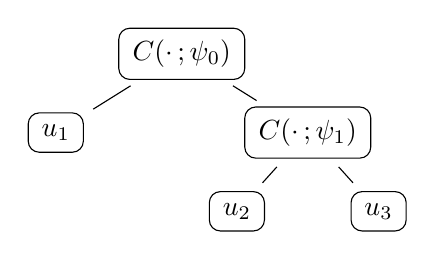
\begin{tikzpicture}[
		    grow=south,
		    level 1/.style={sibling distance=32mm,level distance=10mm},
		    level 2/.style={sibling distance=18mm,level distance=10mm},
		    edge from parent/.style={draw,shorten >=1.4mm,shorten <=1.4mm},
		    every node/.style={draw,rectangle,rounded corners,inner sep=0mm},
				mynodestyle/.style={minimum width=16mm,minimum height=6.5mm},
				myleafstyle/.style={minimum width=7mm,minimum height=5mm}
		    ]
			\node[mynodestyle]{$C(\cdot\,;\psi_0)$}
			   %left
			    child{
			       node[myleafstyle]{$u_1$}
			    }
			   %right
			    child{
			      node[mynodestyle]{$C(\cdot\,;\psi_1)$}{
			      	%left
							child{
								node[myleafstyle]{$u_2$}
							}
							%right
							child{
								node[myleafstyle]{$u_3$}
							}
			      }
			    };
  \end{tikzpicture}
  \setcapwidth{\textwidth}%
  \caption{Tree structure of a three-dimensional fully nested Archimedean copula.}
  \label{fig:NAC_3d}
\end{figure}
Due to this tree representation, we refer to the outermost Archimedean copula
generated by $\psi_0$ as \textit{root copula}. We refer to Archimedean
copulas on an innermost nesting level, i.e., Archimedean copulas that
contain at least one argument which is not a nested Archimedean copula, as
\textit{leaf copulas}. Further, we call an Archimedean copula appearing in the
tree structure of a nested Archimedean copula \textit{parent copula} if it is a
nested Archimedean copula with at least one nested Archimedean copula as one of
its components. We refer to these components as \textit{child copulas}.

In \R, because of the recursive tree structure, a powerful approach is to
use a \emph{recursive} class definition: In the \pkg{nacopula} package, we
define the \code{nacopula} (\textbf{n}ested \textbf{a}rchimedean
\textbf{copula}) class, with three components (\code{slots}),
\begin{Schunk}
%% manual cut & paste from ../../R/AllClass.R :
\begin{Sinput}
setClass("nacopula",
	 representation(copula    = "acopula",
                        comp      = "integer",  # from 1:d -- of length in [0,d]
                        childCops = "list" # of nacopulas, possibly empty
                       ),
         validity = function(object) {
            ......
             if(!all("nacopula" == sapply(object@childCops, class)))
                 return("All 'childCops' elements must be 'nacopula' objects")
            ......
         })
\end{Sinput}
\end{Schunk}
i.e., by its root copula (slot \code{@ copula}, a \code{"acopula"} object),
a vector of indices of its ``direct components'' (slot \code{ @comp = 1 }
for $u_1$ in the example), and a list of child copulas (slot \code{@ childCops}).
The \code{outer_nacopula} is a version of the \emph{same} class (i.e., it
``contains'' \code{nacopula} without any further slots), just with
stricter validity checking, namely requiring that all components from all
child copulas are exactly the set $\{1,2,\dots,d\}$.
\begin{Schunk}
\begin{Sinput}
setClass("outer_nacopula", contains = "nacopula",
         validity = function(object) {
             ## *Extra* checks in addition to those of "nacopula"
             .......
        })
\end{Sinput}
\end{Schunk}
For example, (one parametrization of) the three-dimensional example from
Figure~\ref{fig:NAC_3d} is
\begin{Schunk}
\begin{Sinput}
> C3 <- onacopula("A", C(0.2, 1, C(0.8, 2:3)))
> C3
\end{Sinput}
\begin{Soutput}
Nested Archimedean copula ("outer_nacopula"), with slot 
'comp'   = (1)  and root
'copula' = Archimedean copula ("acopula"), family "AMH", theta= (0.2)
and 1 child copula
   Nested Archimedean copula ("nacopula"), with slot 
   'comp'   = (2, 3)  and root
   'copula' = Archimedean copula ("acopula"), family "AMH", theta= (0.8)
   and *no* child copulas
\end{Soutput}
\begin{Sinput}
> ## and the above is shortened from
> stopifnot(identical(C3,
+       onacopula("A", C(0.2, 1, list(C(0.8, 2:3, list()))))
+ ))
\end{Sinput}
\end{Schunk}

The recursive definition (\ref{nac}) of nested Archimedean copulas not only leads to
recursive class definitions in \R, but also to recursive functions for
computing on such ``nacopulas''.
All the following functions and methods (from our package \code{nacopula})
are defined \emph{recursively}, typically using
\code{lapply(x @ childCops,} \textit{<fun>}\code{)}:
The utilities \code{dim()}, \code{allComp()}, \code{printNacopula()} (which is the hidden
\code{show()} method), and the principal functions
\code{pnacopula()} and \code{rncopula()} (via recursive utility \code{rnchild()}.
As a simple example of these, \code{pnacopula(x, u)} simply evaluates the
(recursive) formula~(\ref{nac}), recursively applying itself to its child copulas:
%% This is not as nice (wrong indentation; lost comments):
% <<pnacopula-def>>=
% pnacopula
% @
%% as this --- cut & paste from ../../R/nacopula.R :
\begin{Schunk}
\begin{Sinput}
pnacopula <- function(x,u) {
    stopifnot(is.numeric(u), 0 <= u, u <= 1, length(u) >= dim(x)) # can be larger
    C <- x@copula
    th <- C@theta
    ## use u[j] for the direct components 'comp':
    C@psi(sum(unlist(lapply(u[x@comp], C@psiInv, theta=th)),
              C@psiInv(unlist(lapply(x@childCops, pnacopula, u = u)),
                       theta=th)),
          theta=th)
}
\end{Sinput}
\end{Schunk}


In order for (\ref{nac}) being indeed a proper copula,
\textcite[p.\ 88]{joe1997} and \textcite{mcneil2008} present the sufficient
\textit{nesting condition} that $\psiis{i}\circ\psi_{j}$ is completely
monotone for all nodes (with parent $i$, child $j$) appearing in a nested
Archimedean copula.
%%
This condition can be derived from a mixture representation of $C$ based on
the distribution functions $F_0:=\LSi[\psi_0]$ and
$F_{ij}:=\LSi[\psi_{ij}(\cdot\,;V_0)]$ for
%$\psi_{ij}(t;x):=\exp\bigl(-x\psiis{i}(\psi_{j}(t))\bigr)$,
\begin{equation*}
  \psi_{ij}(t;x):=\exp\bigl(-x\psiis{i}(\psi_{j}(t))\bigr),
\end{equation*}
$x\in(0,\infty)$.

\subsection{Sampling}
If the nesting condition is fulfilled for all %% appearing
nodes in the nested Archimedean structure, the
following algorithm may be derived for sampling nested Archimedean copulas.
\begin{algorithm}
  Let $C$ be a nested Archimedean copula with root copula $C_0$ generated by
  $\psi_0$. Let $\bm{U}$ be a vector of the same dimension as $C$.
  \myskipalgotext
  \linespread{1.22}\normalfont
  \begin{tabbing}
	\hspace{8mm} \= \hspace{4mm} \= \kill
	(1) \> \textbf{sample} $V_0\sim F_0=\LSi[\psi_0]$\\
	(2) \> \textbf{for} all components $u$ of $C_0$ that are nested
	 Archimedean copulas \textbf{do} \{\\
	(3) \>\> \textbf{set} $C_1$ with generator $\psi_1$ to be the nested
	 Archimedean copula $u$\\
	(4) \>\> \textbf{sample} $V_{01}\sim F_{01}=\LSi[\psi_{01}(\cdot\,;V_0)]$\\
	(5) \>\> \textbf{set} $C_0:=C_1$, $\psi_0:=\psi_1$, and $V_0:=V_{01}$ and \textbf{continue} with (2)\\
	(6) \> \}\\
	(7) \> \textbf{for} all other components $u$ of $C_0$ \textbf{do} \{\\
	(8) \>\> \textbf{sample} $R\sim\Exp(1)$\\
	(9) \>\> \textbf{set} the component of $\bm{U}$ corresponding to $u$
	 to $\psi_0(R/V_0)$\\
	(10) \> \}\\
	(11) \> \textbf{return} $\bm{U}$
   \end{tabbing}
\end{algorithm}
Note that for sampling nested Archimedean copulas when all generators
involved belong to the same parametric family, it suffices to know how to
sample
\begin{align*}
  V_0\sim F_0=\LSi[\psi_0],\quad F_{01}=\LSi[\psi_{01}(\cdot\,;V_0)]
\end{align*}
as all distribution functions $F_{ij}$ take the same form as $F_{01}$, only
the parameters may differ.
In our \R{} package \pkg{nacopula}, the supported Archimedean family
objects therefore provide the three slots \code{V0}, \code{nestConstr} and \code{V01},
all functions. \code{nestConstr}, is a
\code{function(}$\theta_0$\code{, }$\theta_1$\code{)} returning \code{TRUE}
when the nesting condition is fulfilled, and \code{V0} and \code{V01} are
random number generating functions, generating
$V$ from Table~\ref{tab:cop-families-psi} and
$V_{01}$ from Table~\ref{tab:nestedAC-V01}, respectively,
e.g., for the most simple case, Ali-Mikhail-Haq,
\begin{Schunk}
\begin{Sinput}
> copAMH @ nestConstr
\end{Sinput}
\begin{Soutput}
function (theta0, theta1) 
{
    copAMH@paraConstr(theta0) && copAMH@paraConstr(theta1) && 
        theta1 >= theta0
}
<environment: namespace:nacopula>
\end{Soutput}
\begin{Sinput}
> copAMH @ V01
\end{Sinput}
\begin{Soutput}
function (V0, theta0, theta1) 
{
    rnbinom(length(V0), V0, (1 - theta1)/(1 - theta0)) + V0
}
<environment: namespace:nacopula>
\end{Soutput}
\end{Schunk}
Sampling strategies for $F_0$ and $F_{01}$ for
many known Archimedean generators are presented in \textcite{hofert2008},
\textcite{hofert2010a}, and \textcite{hofert2010c}. For the families of
Ali-Mikhail-Haq, Clayton, Frank, Gumbel, and Joe, Table~\ref{tab:nestedAC-V01}
summarizes stochastic representations for $V_0$ and $V_{01}$.
\begin{table}[htbp]
  \centering
  \begin{tabularx}{\textwidth}{@{\extracolsep{\fill}}X>{\hspace{-7mm}}c>{\hspace{-8mm}}c}
	\toprule
	\multicolumn{1}{c}{Family}&\multicolumn{1}{c}{\hspace{-7mm}nesting condition}
        &\hspace{-8mm}$V_{01}\sim F_{01}=\LSi[\psi_{01}(\cdot\,;V_0)]$\\
	\midrule
	Ali-Mikhail-Haq&$\vt_0\le\vt_1$&$V_0+X$, $X\sim\NB(V_0,(1-\vt_1)/(1-\vt_0))$\\
	Clayton&$\vt_0\le\vt_1$&$\tS(\vt_0/\vt_1,1,(\cos(\pi\vt_0/(2\vt_1))V_0)^{\vt_1/\vt_0},V_0\I_{\{\vt_0=\vt_1\}},\I_{\{\vt_0\neq\vt_1\}};1)$\\
	Frank&$\vt_0\le\vt_1$&$\sum_{j=1}^{V_0}V_j$; for $V_j$, see \textcite{hofert2010a}\\
	Gumbel&$\vt_0\le\vt_1$&$\S(\vt_0/\vt_1,1,(\cos(\pi\vt_0/(2\vt_1))V_{0})^{\vt_1/\vt_0},\I_{\{\vt_0=\vt_1\}};1)$\\
	Joe&$\vt_0\le\vt_1$&$\sum_{j=1}^{V_0}V_j$; $V_j\sim\binom{\alpha}{k}(-1)^{k-1},\ k\in\IN$\\
	\bottomrule
   \end{tabularx}
   \caption{Nesting conditions and stochastic representations for $V_{01}$
     (see also comments below).}
   \label{tab:nestedAC-V01}
\end{table}

First note that for nested Archimedean copulas based on generators belonging to
the same Archimedean family, all implemented families indeed lead to proper
copulas if the generators on a more nested (inner) level have larger parameter
values than the ones on a lower (outer) level. This is equivalent to saying that
Kendall's tau for a pair of random variables having an Archimedean copula
which resides on a deeper nesting level as common margin has to be larger than
or equal to the one for a pair of random variables having an Archimedean
marginal copula residing on a lower nesting level.
Slightly more informally, the inner (or lower) nested components $u_j$ are
\emph{more} correlated than the outer (``higher up'') ones.

Some comments on the distributions $F_{01}$ of $V_{01}$ for the
different implemented families: For the family of Ali-Mikhail-Haq, $V_{01}$
admits the stochastic representation $V_0+X$, where $X$ follows a negative
binomial distribution with parameters as given in Table~\ref{tab:nestedAC-V01}. The
parameterization is $\NB(r,p)$, $r\in(0,\infty)$, $p\in(0,1)$, with mass
function $p_k=\binom{k+r-1}{r-1}p^r(1-p)^k$, $k\in\IN_0$, which in \R{} is
\code{dnbinom(}$k$\code{, size=}$r$\code{, prob=}$p$\code{)}.
%% dnbinom(x, size, prob, mu, log = FALSE)

For Clayton's family, $F_{01}$ can be interpreted as a special case (take
$h:=1$, $\alpha:=\vt_0/\vt_1$) of the \textit{exponentially tilted stable
  distribution}
\begin{align}
  \tS(\alpha,1,(\cos(\alpha\pi/2)V_0)^{1/\alpha},V_0\I_{\{\alpha=1\}},h\I_{\{\alpha\neq1\}};1)\label{exptilted}
\end{align}
with $\alpha\in(0,1]$, $h\in[0,\infty)$, and $V_0\in(0,\infty)$, and
corresponding Laplace-Stieltjes transform
\begin{align*}
  \psi(t)=\exp\bigl(-V_0((h+t)^{\alpha}-h^{\alpha})\bigr),\ t\in[0,\infty].
\end{align*}
\textcite{hofert2010a} suggested a fast rejection algorithm for sampling this
distribution. \textcite{devroye2009} suggested an algorithm for
sampling the exponentially tilted stable distribution
\begin{align*}
  \tS(\alpha,1,\cos(\alpha\pi/2)^{1/\alpha},\I_{\{\alpha=1\}},\lambda\I_{\{\alpha\neq1\}};1)
\end{align*}
with $\alpha\in(0,1]$ and $\lambda\in[0,\infty)$, and corresponding
Laplace-Stieltjes transform
\begin{align*}
  \psi(t)=\exp\bigl(-((\lambda+t)^{\alpha}-\lambda^{\alpha})\bigr),\ t\in[0,\infty].
\end{align*}
One can easily check that by setting $\lambda:=hV_0^{1/\alpha}$ and
generating $V_\lambda$ with the algorithm of \textcite{devroye2009}, the
random variable $V_{01}$ from $F_{01}$ as given by (\ref{exptilted}) can be
obtained via $V_{01}=V_0^{1/\alpha}V_\lambda$. Therefore, the distribution as
given in (\ref{exptilted}) may be sampled by either the algorithm of
\textcite{devroye2009} or the one of \textcite{hofert2010a}. The former
author reports that the complexity of his algorithm is bounded, the latter
author shows that the complexity of his algorithm is $\O(V_{0}h^{\alpha})$.
We implemented both algorithms for sampling (\ref{exptilted}) in the package
\pkg{nacopula} and decide for each drawn $V_0$ which method is to be
applied. As a simple rule, investigated by several parameter combinations,
the default chooses the method of \textcite{hofert2010a} if
$V_{0}h^{\alpha}<4$ and the one of \textcite{devroye2009} otherwise. As
mentioned before, note that for sampling nested Clayton copulas, we have
$h=1$. Further, $\IE[V_0]=1/\vt_0$. Hence, in the mean, the algorithm of
\textcite{hofert2010a} is more often applied if $\vt_0>1/4$,
equivalently, if Kendall's tau for the bivariate Archimedean copula
generated by $\psi_0$ is greater than $1/9$.

For Frank's family, \textcite{hofert2010a} presented a rejection algorithm.
For the family of Gumbel, $\psi_{01}(t;V_0)=\exp(-V_0t^\alpha)$,
$\alpha:=\vt_0/\vt_1$, hence, see Table~\ref{tab:cop-families-psi}, $F_{01}$ corresponds
to the stable distribution as given in Table~\ref{tab:nestedAC-V01}. Finally, for
Joe's Archimedean family, $V_{01}$ can be represented as a $V_0$-fold sum of
independent and identically distributed random variables $V_k$,
$k\in\{1,\dots,V_0\}$, from the same distributional class as $V_0$, see
Table~\ref{tab:cop-families-psi}. For more information on the distributions of $V_{01}$,
see \textcite{hofert2010a} and \textcite{hofert2010c}, or the source code of
the package \pkg{nacopula}.

\subsection{A nine-dimensional nested Clayton copula}
In this example, we consider a nine-dimensional partially nested Archimedean
copula $C$ of the form
\begin{align*}
 C(\bm{u})=C(u_3,u_6,u_1,C(u_9,u_2,u_7,u_5,C(u_8,u_4;\psi_2);\psi_1);\psi_0)
\end{align*}
with tree structure depicted in Figure~\ref{figure2}.
\begin{figure}[htbp]
 \centering
 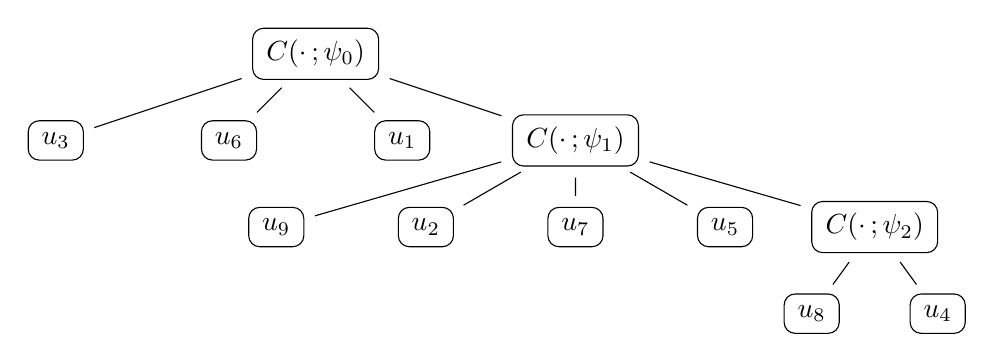
\begin{tikzpicture}[
	grow=south,
  	level 1/.style={sibling distance=22mm,level distance=11mm},
  	level 2/.style={sibling distance=19mm,level distance=11mm},
  	level 3/.style={sibling distance=16mm,level distance=11mm},
  	edge from parent/.style={draw,shorten >=1.4mm,shorten <=1.4mm},
  	every node/.style={draw,rectangle,rounded corners,inner sep=0mm},
	mynodestyle/.style={minimum width=16mm,minimum height=6.5mm},
	myleafstyle/.style={minimum width=7mm,minimum height=5mm}
  ]
\node[mynodestyle]{$C(\cdot\,;\psi_0)$}
  %child 0,1
  child{
     node[myleafstyle]{$u_3$}
   }
 %child 0,2
  child{
     node[myleafstyle]{$u_6$}
   }
 %child 0,3
  child{
     node[myleafstyle]{$u_1$}
   }
  %child 0,4
   child{
     node[mynodestyle]{$C(\cdot\,;\psi_1)$}{
     	%child 1,1
			child{
				node[myleafstyle]{$u_9$}
			}
			%child 1,2
			child{
				node[myleafstyle]{$u_2$}
			}
			%child 1,3
			child{
				node[myleafstyle]{$u_7$}
			}
			%child 1,4
			child{
				node[myleafstyle]{$u_5$}
			}
			%child 1,5
			child{
				node[mynodestyle]{$C(\cdot\,;\psi_2)$}
				%child 2,1
				child{
					node[myleafstyle]{$u_8$}
				}
				%child 2,2
				child{
					node[myleafstyle]{$u_4$}
				}
			}
     }
   };
\end{tikzpicture}
\setcapwidth{\textwidth}%
\caption{Tree structure of the nine-dimensional partially nested Archimedean
copula $C$.}
\label{figure2}
\end{figure}
Such a copula can be defined as follows, where we choose the parameters of
$\psi_0$, $\psi_1$, and $\psi_2$ such that the corresponding Kendall's taus are
0.2, 0.5, and 0.8, respectively.
\begin{Schunk}
\begin{Sinput}
> theta0 <- copClayton@tauInv(0.2)
> theta1 <- copClayton@tauInv(0.5)
> theta2 <- copClayton@tauInv(0.8)
> c(theta0, theta1, theta2)
\end{Sinput}
\begin{Soutput}
[1] 0.5 2.0 8.0
\end{Soutput}
\begin{Sinput}
> C_9_clayton <- onacopula("Clayton",
+                          C(theta0, c(3,6,1),
+                            C(theta1, c(9,2,7,5),
+                              C(theta2, c(8,4)))))
> C_9_clayton # show(.) it
\end{Sinput}
\begin{Soutput}
Nested Archimedean copula ("outer_nacopula"), with slot 
'comp'   = (3, 6, 1)  and root
'copula' = Archimedean copula ("acopula"), family "Clayton", theta= (0.5)
and 1 child copula
   Nested Archimedean copula ("nacopula"), with slot 
   'comp'   = (9, 2, 7, 5)  and root
   'copula' = Archimedean copula ("acopula"), family "Clayton", theta= (2)
   and 1 child copula
      Nested Archimedean copula ("nacopula"), with slot 
      'comp'   = (8, 4)  and root
      'copula' = Archimedean copula ("acopula"), family "Clayton", theta= (8)
      and *no* child copulas
\end{Soutput}
\end{Schunk}

Let us sample 500 random variates (each in $[0,1]^9$) from this copula
(this involves our efficient procedure for exponentially tilted stable
distributions) and visualize the generated data with a scatter-plot matrix.
\begin{Schunk}
\begin{Sinput}
> set.seed(1)
> dim(U9 <- rnacopula(500, C_9_clayton))
\end{Sinput}
\begin{Soutput}
[1] 500   9
\end{Soutput}
\begin{Sinput}
> ## For plotting, re-order the columns according to the same strength
> ## of dependence:
> j <- allComp(C_9_clayton)
> (vnames <- do.call(expression,
+                    lapply(j, function(i) substitute( U[I], list(I=0+i)))))
\end{Sinput}
\begin{Soutput}
expression(U[3], U[6], U[1], U[9], U[2], U[7], U[5], U[8], U[4])
\end{Soutput}
\begin{Sinput}
> print(splom2(U9[, j], varnames= vnames,
+              cex = 0.4, pscales = 0))
\end{Sinput}
\end{Schunk}
\includegraphics{nacopula-ex2-splom}

The population version of Kendall's tau for $(U_4,U_5)\tr$ is 0.5. Let us check
if the sample version of Kendall's tau is close to this value.
\begin{Schunk}
\begin{Sinput}
> round(cor(U9[,9],U9[,7], method="kendall"), 3)
\end{Sinput}
\begin{Soutput}
[1] 0.5
\end{Soutput}
\end{Schunk}

Evaluating this nine-dimensional nested Clayton copula at
$(0.5,\dots,0.5)\tr$ and near the upper corner $(0.99,\dots,0.99)\tr$ leads to
the following results.
\begin{Schunk}
\begin{Sinput}
> c(pnacopula(C_9_clayton, rep(.5,9)),
+   pnacopula(C_9_clayton, rep(.99,9)))
\end{Sinput}
\begin{Soutput}
[1] 0.09375995 0.91747302
\end{Soutput}
\end{Schunk}

The probability mass in the cube  $(0.8, 1]^9$ can be determined as follows.
\begin{Schunk}
\begin{Sinput}
> prob(C_9_clayton, rep(.8,9), rep(1,9))
\end{Sinput}
\begin{Soutput}
[1] 0.001061674
\end{Soutput}
\end{Schunk}

Finally, let us find the different lower and upper tail-dependence coefficients
appearing on different levels for this nested Archimedean copula.
\begin{Schunk}
\begin{Sinput}
> c(copClayton @ lambdaL(theta0),
+   copClayton @ lambdaU(theta0))
\end{Sinput}
\begin{Soutput}
[1] 0.25 0.00
\end{Soutput}
\begin{Sinput}
> c(copClayton @ lambdaL(theta1),
+   copClayton @ lambdaU(theta1))
\end{Sinput}
\begin{Soutput}
[1] 0.7071068 0.0000000
\end{Soutput}
\begin{Sinput}
> c(copClayton @ lambdaL(theta2),
+   copClayton @ lambdaU(theta2))
\end{Sinput}
\begin{Soutput}
[1] 0.917004 0.000000
\end{Soutput}
\end{Schunk}

\section{Outer power Archimedean copulas}
For an Archimedean generator $\psi\in\Psi_\infty$, $\psi(t^{1/\vt})$ is also a
valid generator in $\Psi_\infty$ for all $\vt\in[1,\infty)$, see, e.g.,
\textcite[p.\ 441]{feller1971}. The resulting copulas are
referred to as \textit{outer power Archimedean copulas}. Note that two
parametric Archimedean generators $\psi(t^{1/\vt_0})$, $\vt_0\in[1,\infty)$, and
$\psi(t^{1/\vt_1})$, $\vt_1\in[1,\infty)$, of this type, constructed with the
same ``base'' generator $\psi(t)$, $t\in[0,\infty)$, fulfill the nesting
condition if $\vt_0\le\vt_1$. Therefore, one can build so-called
\textit{nested outer power Archimedean copulas}.
\textcite{hofert2010a} derives some results for
these copulas, including instructions for sampling the corresponding random
variables $V_0$ and $V_{01}$, as well as an explicit formula for Kendall's tau
in terms of the Kendall's tau of the copula generated by the base generator
$\psi$. Further, note that if the tail-dependence coefficients exist, they are
greater than or equal to the ones corresponding to the base generator.
For the Archimedean families implemented in the package \pkg{nacopula}, these
can all be computed explicitly.

The goal of this section is to show how one might work with outer power
Archimedean copulas with the package \pkg{nacopula}.
For now, we use the outer power transformation \code{opower()}
which generates an outer power family based on the provided copula family
\code{copbase} with corresponding parameter \code{thetabase}.
\begin{Schunk}
\begin{Sinput}
> str(opower)
\end{Sinput}
\begin{Soutput}
function (copbase, thetabase)  
\end{Soutput}
\end{Schunk}
We believe that it is both more natural and flexible
to work with copula families that are \emph{generalizations} of our current
families, each including the power as an extra parameter (such that
\code{theta}, i.e., $\vartheta$, will become 2-dimensional), rather than
using the \code{opower()} construction below. This section therefore should be
considered mainly as an outlook to further features of the package
\pkg{nacopula}, where this transformation is not required anymore for working
with outer power Archimedean copulas.

Using this transformation, we define a valid outer power Clayton copula with
base generator of Clayton's type and with base parameter such that Kendall's tau
equals 0.5.
%% MM: chosing name "opow.Clayton"  to make it "stand out":
\begin{Schunk}
\begin{Sinput}
> thetabase <- copClayton@tauInv(.5)
> (opow.Clayton <- opower(copClayton, thetabase))
\end{Sinput}
\begin{Soutput}
Archimedean copula ("acopula"), family "opower:Clayton"
 It contains further slots, named
  "psi", "psiInv", "paraConstr", "paraInterval", "V0", "tau",
  "tauInv", "lambdaL", "lambdaLInv", "lambdaU", "lambdaUInv",
  "nestConstr", "V01"
\end{Soutput}
\end{Schunk}

Based on this copula generator, we would like to define and sample a
three-dimensional fully nested outer power Clayton copula with parameters
such that Kendall's tau are $2/3$ and $0.75$.
%% onacopula() now works since Martin implemented it on 2010-06-26  :
\begin{Schunk}
\begin{Sinput}
> theta0 <- opow.Clayton@tauInv(2/3) # should be 1.5
> theta1 <- opow.Clayton@tauInv(.75) # should be 2
> ## Define a 3d fully nested Archimedean copula based on  opow.Clayton
> opC3 <- onacopula(opow.Clayton, C(theta0, 1, C(theta1, c(2,3))))
\end{Sinput}
\end{Schunk}

Now sample 500 random variates from this copula and visualize the generated
data with a scatter-plot matrix. In contrast to Clayton copulas, note that
this outer power Clayton copula has both lower and upper tail dependence.
%% dim(U3 <- rnacopula(500, opC3))
\begin{Schunk}
\begin{Sinput}
> U3 <- rnacopula(500, opC3) ; stopifnot(dim(U3) == c(500,3))
> print( splom2(U3, cex = 0.4) )
\end{Sinput}
\end{Schunk}
\includegraphics{nacopula-opower-splom}

Further, we can compare the population and sample versions of Kendall's tau for
the generated data. The $(1,2)$- and $(1,3)$-entry of the matrix of
pairwise sample versions of Kendall's tau should be close to $2/3$, the
$(2,3)$-entry should be close to $0.75$.
\begin{Schunk}
\begin{Sinput}
> round(cor(U3, method="kendall"), 3)
\end{Sinput}
\begin{Soutput}
      [,1]  [,2]  [,3]
[1,] 1.000 0.663 0.644
[2,] 0.663 1.000 0.764
[3,] 0.644 0.764 1.000
\end{Soutput}
\end{Schunk}

The different lower and upper tail-dependence coefficients for this copula can
be obtained as follows.
\begin{Schunk}
\begin{Sinput}
> rbind(th.0 =
+       c(L = opow.Clayton @ lambdaL(theta0),
+         U = opow.Clayton @ lambdaU(theta0)),
+       th.1 =
+       c(L = opow.Clayton @ lambdaL(theta1),
+         U = opow.Clayton @ lambdaU(theta1)))
\end{Sinput}
\begin{Soutput}
             L         U
th.0 0.7937005 0.4125989
th.1 0.8408964 0.5857864
\end{Soutput}
\end{Schunk}

%%   =======

\section{Session Info}

\begin{Schunk}
\begin{Sinput}
> toLatex(sessionInfo())
\end{Sinput}
\begin{itemize}\raggedright
  \item R version 2.11.1 Patched (2010-07-01 r52421), \verb|x86_64-unknown-linux-gnu|
  \item Locale: \verb|LC_CTYPE=de_CH.UTF-8|, \verb|LC_NUMERIC=C|, \verb|LC_TIME=en_US.UTF-8|, \verb|LC_COLLATE=de_CH.UTF-8|, \verb|LC_MONETARY=C|, \verb|LC_MESSAGES=de_CH.UTF-8|, \verb|LC_PAPER=de_CH.UTF-8|, \verb|LC_NAME=C|, \verb|LC_ADDRESS=C|, \verb|LC_TELEPHONE=C|, \verb|LC_MEASUREMENT=de_CH.UTF-8|, \verb|LC_IDENTIFICATION=C|
  \item Base packages: base, datasets, graphics, grDevices,
    methods, stats, tools, utils
  \item Other packages: lattice~0.18-8, nacopula~0.4-2
  \item Loaded via a namespace (and not attached):
    grid~2.11.1, gsl~1.9-3
\end{itemize}\end{Schunk}
%%
%% packageDescription("nacopula")[c("Version", "LastChanged")]
%% Now,  packageDescription("nacopula")[["LastChanged"]]  is too long,
%% ----> we "cheat" as follows:
\begin{Schunk}
\begin{Sinput}
> my.strsplit(  packageDescription("nacopula")[["LastChanged"]]  )
\end{Sinput}
\end{Schunk}
\begin{Schunk}
\begin{Soutput}
$LastChangedRevision: 226 $
$LastChangedDate: 2010-07-02 09:41:53 +0200 (Fri, 02. Jul 2010) $
\end{Soutput}
\end{Schunk}

\section{Conclusion}
The package \pkg{nacopula} allows to easily construct and work with nested
Archimedean copulas. First and foremost, fast sampling algorithms for these copulas
are implemented. As a by-product, the package also provides related mathematical
and random number generating functions, e.g., an efficient
sampling algorithm for exponentially tilted stable distributions. Further
features include the evaluation of nested Archimedean copulas, as well as
computing probabilities of a random vector falling into a given hypercube.
Concerning measures of association, Kendall's tau and the tail-dependence
coefficients are implemented. Currently supported Archimedean families include
the well-known families of Ali-Mikhail-Haq, Clayton, Frank, Gumbel, and Joe.

\bibliography{mh-biblio}

\end{document}
